\documentclass[12pt, a4paper]{article}

\usepackage{xeCJK}  % xelatex 中文
\setCJKmainfont{AR PL UMing CN}
\usepackage{titling}
\setlength{\droptitle}{-4cm}
\usepackage{graphicx}
\graphicspath{ {images/} }

\title{ADLxMLDS 2017 Fall\\HW1 - Sequence Labeling}

\author{B05901189 吳祥叡}
\begin{document}
	{\let\newpage\relax\maketitle}
	\section{Model Description}
		\subsection{RNN Model}
			\begin{figure}[h]
				
\includegraphics[width=\linewidth]{2LayerLSTM.png}
				\caption{兩層的 RNN Model}
			\end{figure}
			圖中縱方向為feature的長度.
			經過兩層RNN layer之後再通過Fully Connected Layer產生frame-wise phone 判斷.
		\subsection{CNN Model}		
			\begin{figure}[h!]
				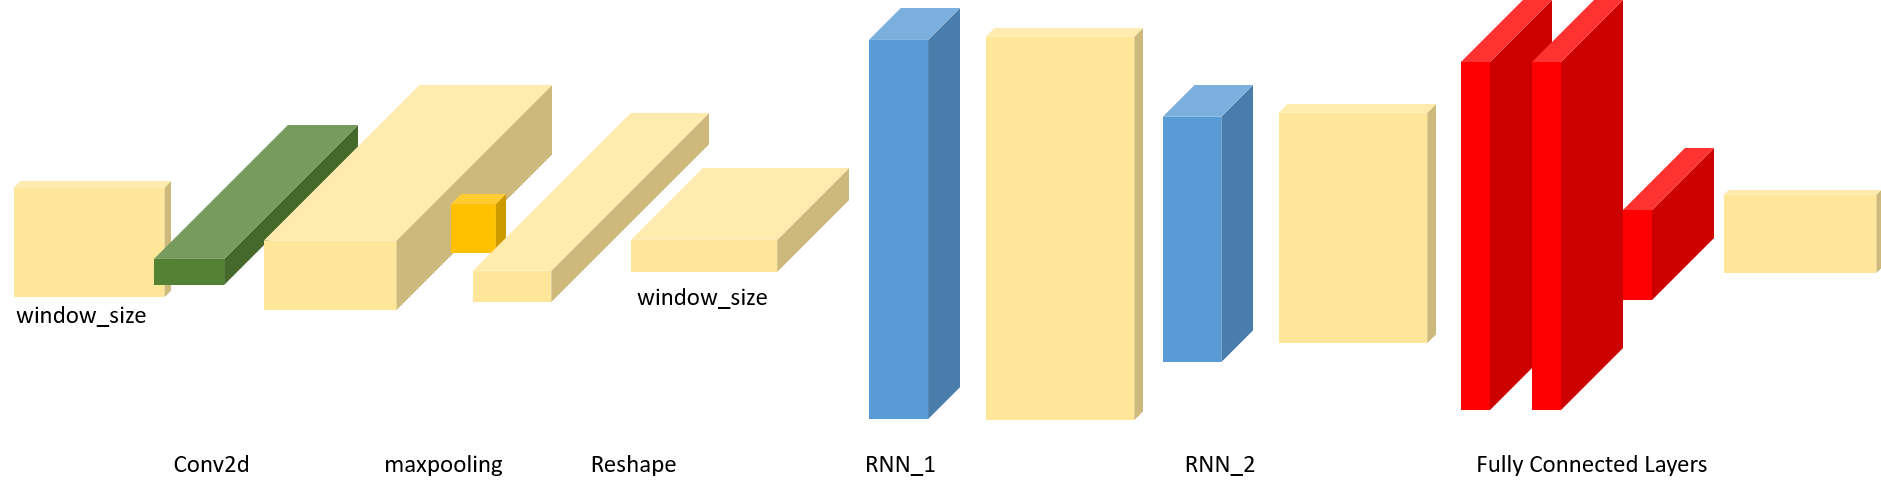
\includegraphics[width=\linewidth]{CNN_model.png}
				\caption{CNN Model}
			\end{figure}
			CNN Model的後半部和RNN Model一樣.前段使用兩個convolution layer和maxpooling layer, 為了把其中一個dimension變成window size要再做reshape.我覺得對時間軸maxpooling可能丟失太多資訊所以也試過沒有maxpooling, 但效果比較不好.
	\section{Boosting Performance}
		\subsection{後處理}
			\begin{enumerate}
			\item 用sliding window 做投票 : 
				因為這些model只能根據一段固定長度的context window對每個frame做預測, 因此我讓window一次只往前移動一個frame再做預測,這樣每個frame就可以有window size次的投票.
			\item 忽略前段和後段的投票 :\\ 
				因為前段和後段可能因為沒有看到比較多前後文所以我選擇忽略掉他們的投票.我做了三次實驗:\\ 
				如果不忽略 :		 kaggle分數 23\\
				前後各忽略10個 :   kaggle分數 20\\
				前後各忽略20個 :   kaggle分數和忽略10個一樣
			\item 去除glich :\\
				我對training data做過統計發現每個phone最少都會由3個frame組成,
				所以決定在把frame-wise prediction 變成phone sequence的時候刪掉小於3個frame的phone.
				如果不刪掉的話kaggle分數20, 用了這個trick可以直接進步到12分.
				或許用seq2seq方法做trimming可以有更好的結果.
			\end{enumerate}
	\section{Experiment Settings and Results}
		\subsection{Experiment Settings}
			\begin{enumerate}
				\item 運算資源 : 有兩個 K80 GPU 的 Azure NC6 
				\item 使用套件 : Tensorflow
				\item 前處理 : 
					將全部timit dataset串起來以便之後產生batch
				\item Validation: 把串好的training data切出後10\%.
				\item Kaggle Metric : 
					每段聲音的平均Phone Error (Edit Distance), 非平常的Phone Error Rate.
			\end{enumerate}
		\subsection{參數試驗}
			\begin{enumerate}
				\item 不同RNN cell: BasicGRU和BasicLSTM Cell表現都差不多
				\item RNN 層數: 發現2層的收歛性比較好
				\item Bidirection: 
				為了比較固定參數量兩種model的表現, 在使用Bidirection的時候的RNN latent dimension都是正常的一半.出乎意料的就算在RNN model, 用Bidirectional RNN完全沒有提昇表現.
				\item Window Size :
				實驗發現32以下的window size在validation acc和loss表現比較不好.超過50之後表現都差不多.原因應該就和要刪除前段和後段類似.
				\item 刪掉不確定的prediction :
				因為原本的prediction是沒有正規化的,所以我取通過softmax機率加總為一的prediction, 設定不同的threshold, 刪掉不確定的prediction. 實驗發現表現都沒有刪除前段和後段的方法好.
			\end{enumerate}
		\subsection{Results}
			\begin{tabular}{|l|c|c|}
				\hline
									& RNN model & CNN model \\\hline
				Validation Loss		& 0.98 		& 0.83 		\\\hline 
				Validation Accuracy	& 69 \% 	& 72 \% 	\\\hline
				Kaggle Public Score & 12.2 		& 9.6 		\\\hline
			\end{tabular}\\\\
			兩種model大約都花一個小時就訓練完, 但也代表這兩個model都很快就overfit, 是一個待解決的問題.
		
		
\end{document}